% (c) Copyright 2017 Josh Wright
\documentclass[12pt]{article}
\usepackage{verbatim}
% \usepackage{syntonly}
\usepackage{ragged2e}
\usepackage{geometry}
\usepackage{enumitem} % for longenum
\usepackage{setspace}
\usepackage{hyperref}
\usepackage{tabularx}
\usepackage{graphicx}
\usepackage{outlines} % for outline
\usepackage{paralist} % for compactitem (compact itemize)
\usepackage{multicol} % for multicolumn layout
\geometry{letterpaper, margin=0.4in, top=0.2in}
% \geometry{letterpaper, margin=0.5in, top=0.35in, left=1.5in}
\pagenumbering{gobble}
\begin{document}
\begin{spacing}{0.8}
%%%%%%%%%%%%%%%%%%
%% main section %%
%%%%%%%%%%%%%%%%%%
\begin{multicols*}{2}
\begin{flushleft}
\newlist{longenum}{itemize}{5}
\setlist[longenum,1]{nosep,leftmargin=0.2cm,labelwidth=0px,align=left,label=$\bullet$}
\setlist[longenum,2]{nosep,leftmargin=0.2cm,labelwidth=0px,align=left,label=$\ast$}
\setlist[longenum,3]{nosep,leftmargin=0.2cm,labelwidth=0px,align=left,label=-}
\setlist[longenum,4]{nosep,leftmargin=0.2cm,labelwidth=0px,align=left,label=$\cdot$}
\setlist[longenum,5]{nosep,leftmargin=0.2cm,labelwidth=0px,align=left,label=@}
% \begin{outline}[compactitem]
\begin{outline}[longenum]
%%%%%%%%%%%%%%%%%%%%
%% spacing config %%
%%%%%%%%%%%%%%%%%%%%
% just in case I need even more space
\newlength{\upspacelength}
\setlength{\upspacelength}{0px}
\newcommand{\upspace}{\vspace{\upspacelength}}
% section titles
\newcommand{\zzz}[1]{\upspace \0 \textbf{#1} }
% \newcommand{\zzz}[1]{\0 \hspace{-1.25in} \textbf{#1} \vspace{-10px} }
% makes second-level itemize bullets instead of dashes
% \renewcommand\labelitemii{\labelitemi}
% redefine the sub-headings to inject our space-saver
\let\oldOne\1\let\oldTwo\2\let\oldThree\3\let\oldFour\4
\renewcommand{\1}{\oldOne   \hspace{-6px}}
\renewcommand{\2}{\oldTwo   \hspace{-6px}}
\renewcommand{\3}{\oldThree \hspace{-6px}}
\renewcommand{\4}{\oldFour  \hspace{-6px}}
\small

\noindent ECEN454 Ref Sheet \hfill \textcopyright \space Josh Wright \today

\newcommand{\VDD}{V_{DD}}

\newcommand{\Vt}{V_{t}}
\newcommand{\Vtn}{V_{tn}}
\newcommand{\Vtp}{V_{tp}}

\newcommand{\Vg}{V_{g}}
\newcommand{\Vs}{V_{s}}
\newcommand{\Vd}{V_{d}}
\newcommand{\Vgn}{V_{gn}}
\newcommand{\Vsn}{V_{sn}}
\newcommand{\Vdn}{V_{dn}}
\newcommand{\Vgp}{V_{gp}}
\newcommand{\Vsp}{V_{sp}}
\newcommand{\Vdp}{V_{dp}}

\newcommand{\Vgs}{V_{gs}}
\newcommand{\Vgd}{V_{gd}}
\newcommand{\Vds}{V_{ds}}
\newcommand{\Vgsn}{V_{gsn}}
\newcommand{\Vgdn}{V_{gdn}}
\newcommand{\Vdsn}{V_{dsn}}
\newcommand{\Vgsp}{V_{gsp}}
\newcommand{\Vgdp}{V_{gdp}}
\newcommand{\Vdsp}{V_{dsp}}
% \newcommand{\V}{V_{}}
% \newcommand{\V}{V_{}}

\zzz{Metric Prefixes} \\
\begin{tabular}{|c c l l|}                                   \hline
peta  & P     & $10^{ 15}$ & \hfill 1 000 000 000 000 000 \\ \hline
tera  & T     & $10^{ 12}$ & \hfill     1 000 000 000 000 \\ \hline
giga  & G     & $10^{  9}$ & \hfill         1 000 000 000 \\ \hline
mega  & M     & $10^{  6}$ & \hfill             1 000 000 \\ \hline
kilo  & k     & $10^{  3}$ & \hfill                 1 000 \\ \hline
hecto & h     & $10^{  2}$ & \hfill                   100 \\ \hline
deca  & da    & $10^{  1}$ & \hfill                    10 \\ \hline
one   &       & $10^{ 0 }$ & \hfill       1 \hfill \hfill \\ \hline
deci  & d     & $10^{- 1}$ & 0.1                          \\ \hline
centi & c     & $10^{- 2}$ & 0.01                         \\ \hline
milli & m     & $10^{- 3}$ & 0.001                        \\ \hline
micro & $\mu$ & $10^{- 6}$ & 0.000 001                    \\ \hline
nano  & n     & $10^{- 9}$ & 0.000 000 001                \\ \hline
pico  & p     & $10^{-12}$ & 0.000 000 000 001            \\ \hline
femto & f     & $10^{-15}$ & 0.000 000 000 000 001        \\ \hline
\end{tabular}

\zzz{De Morgan's Laws}
  \1 $\overline{AB}=\overline {A}+\overline{B}$
  \1 $\overline{A+B}=(\overline{A})(\overline{B})$

\zzz{Silicon}
  \1 Si
  \1 P-type:
    \2 doped with material to remove electrons (add electron holes), usually Boron (B), Aluminum (Al), or Gallium (Ga)
  \1 N-type:
    \2 doped with material to add electrons, usually Antimony (Sb), Arsenic (As), or Phosphorous (P)
  \1 Silicon dioxide: SiO$_2$
  \1 Polysilicon is just silicon without the crystal structure

\zzz{Transistors}
  \1 nMOS
    \2 no bubble
    \2 on when input is on, off when input is off
    \2 base (of whole chip) is p-substrate
    \2 spot of n+ for source and drain, joined by a small layer of oxide (SiO$_2$) and polysilicon (gate). also has a spot of p+ (base) connected to ground
  \1 pMOS:
    \2 has the bubble
    \2 on when input is 0, off when input is 1
    \2 whole thing sits in an n-well (inside the p-substrate base)
    \2 source and drain are spots of p+ connected by gate.
      Gate is polysilicon layer separated from rest of chip by thin layer of SiO$_2$ on bottom.
      Also has a n+ spot for base (connected to VDD)
  \1 CMOS: when you combine a nMOS and pMOS network together to make a gate, where one is the compliment of the other
  \1 $V_t$: Threshold voltage. Nominal voltage below which the transistor is off
    \2 below as in closer to 0, not less
    \2 $V_t>0$ for nMOS, $V_t<0$ for pMOS
    \2 this is compared to the gate to source voltage, $V_{gs}$
  \1 regions: (for nMOS)
    \2 accumulation: gate is negatively charged, attracts positive voids in p-substrate, which block flow in the channel
    \2 depletion: small positive charge on gate repels positive voids from channel, forming a depletion below the gate
    \2 inversion: higher positive charge ($>V_t$) is applied to gate, attracting electrons to the channel and allowing flow

\zzz{D Flip Flop vs Latch}
  \1 latch is level triggered
  \1 flip flop is edge triggered

\zzz{Fabrication}
  \1 n-well: use diffusion or ion implantation
  \1 positive lithography: expose to UV where you want to remove material
  \1 negative lithography: expose to UV where you want to keep material



% lecture 4
\zzz{Stick Diagram vs Boolean Function}
  \1 TODO
  \1 there is more than one way of making a stick diagram for an expression
    \2 stuff in series could be in different order, for instance
  \1 if you do it manually, you need to check it with tools:
    \2 LVS: Layout Vs Schematic
    \2 DRC: Design Re-Check
    \2 These aren't really needed for designs automatically generated from verilog code, because of course that's correct

\zzz{Lithography}
  \1 the process of printing onto a chip at nanometer scale
  \1 generally uses UV light, wavelength around 150nm
    \2 must use fancy tricks to make 10nm features with 150nm light
    \2 would be nice to use even lower wavelength X-rays, but those are hard to focus
  \1 negative lithography: use the lithography mask to cover what you want to keep.
  \1 positive lithography: mask what you want to remove
  \1 a lens is used to focus the light
    \2 ideally, want a point source for the light, but that is not practical
    \2 Optical Proximity Effect: what happens when your focus from the lens is not just right
    \2 results in rounded corners, inaccurate critical dimensions, and shorter wire ends
    \2 can use Optical Proximity Correction to fix:
    \\ basically over-emphasize all the features, and/or add extra lines at outset

\zzz{MOS transitive $I$-$V$ Characteristics and Parasitics}
  \1 $I$-$V$: current-voltage relationship
  \1 Transistors are not really ideal switches, they have 3 zones of operation: cutoff, linear, saturation
  \1 definitions:
    \\ $V_{gs}$: voltage gate to source
    \\ $V_{gd}$: voltage gate to drain
    \\ $V_{ds}$: voltage source to drain (across the channel)
    \\ $V_t$: critical voltage at which transistor is saturated
    \\ channel: space between the source and drain, where the electrons flow
  \1 remember that the gate is insulated from the area under it by a thin layer of Silicon Dioxide (SiO$_2$)
  \1 by convention, the source is the terminal at lower voltage
  \1 \textbf{cutoff}:
    \2 when $V_{gs}<0$
    \2 electrons on the gate attract positive voids in the silicon below, and inhibit current flow. Therefore, the transistor is closed.
    \2 $I_{ds}=0$
  \1 \textbf{linear}:
    \2 $V_{gs}>V_t, V_{gd}=V_{gs}, V_{ds}=0$
    or $V_{gs}>V_t, V_{gs}>V_{gd}>V_t, 0<V_{ds}<V_{gs}-V_t$
    \2 $I_{ds}$ linearly proportional to $V_{ds}$
    \2 channel of electrons forms, allowing current to flow
  \1 \textbf{saturated:}
    \2 $V_{gs}>V_t, V_{gd}<V_t, V_{ds}>V_{gs}-V_t$
    \2 channel pinches off due to electrons attracting to source
    \2 $I_{ds}$ is independent of $V_{ds}$
\zzz{capacitor effect}
  \1 gate and channel can have a parallel plate capacitor effect, with the thin layer of SiO$_2$ acting as the insulator
  \1 $C=\frac{Q}{V}=\epsilon_{SiO_2}wl/t_{SiO_2}, V = V+{gc}-V_t=(v_{gs}-V{ds}/2)-V_t$
    \2 $l,w$: length, width of section of gate above channel
    \2 $\epsilon_{SiO_2}$: permittivity of SiO$_2$ layer
    \2 $t_{SiO_2}$: thickness of SiO$_2$ layer
  \1 general capacitance per unit area: $C_{ox}=\frac{\epsilon_{ox}}{t_{ox}}$
    \2 $\epsilon_{ox}$: permittivity of oxidation layer
    \2 $t_{ox}$: thickness of oxidation layer
  \1 carrier velocity: velocity of the electrons?
    \2 proportional to the electric field running horizontally between source and drain
    \2 $v=\mu E, E=V_{ds}/L, t=L/v=L/(\mu E)=L/(\mu\frac{V_{ds}}{L})$
    \\ $\mu$: mobility. electrons move about twice as fast as positive voids
    \\ $L$: length of channel
  \1 actual velocity of electrons is the speed of light, but they don't travel in a straight line, they travel atom-to-atom
    \2 this slowdown is called the \textbf{scattering} effect
\zzz{Shockley model of transistor}
  \1 $V_{dsat}=V_{gs}-V_t$
  \1 1st order model: $\beta=\mu C_{SiO_2}\frac{w}{l}$
  \begin{tabular}{l l l}
  $V_{gs} < V_t     $ & $I_{ds}=0$                                        & cutoff  \\
  $V_{ds} < V_{dsat}$ & $I_{ds}=\beta(V_{gs}-V_t-\frac{V_{ds}}{2})V_{ds}$ & linear \\
  $V_{ds} > V_{dsat}$ & $I_{ds}=\frac{\beta}{2}(V_{gs}-V_t)^2$            & saturation  \\
  \end{tabular}
  \1 Must be able to derive this model on exam!

\zzz{Non-Ideal $I$-$V$ Effects}
  \1 velocity saturation (due to scattering)
    \2 also called short channel effect
    \2 this is hard to make into a mathematical formula
  \1 sub-threshold leakage, junction leakage, gate tunneling
  \1 \textbf{Body Effect}
    \2 affected by $V_{sb}$: voltage of the p-substrate (which should be ground)
    \2 $V_t=V_{t0}+\lambda(\sqrt{|-2\phi_F+V_{sb}|}-\sqrt{|-2\phi_F|})$
      \3 $V_{t0}$: threshold without body bias
      \3 $\phi_F$: Fermi potential
        \4 negative for nMOS, positive for pMOS
      \3 $\lambda$: body effect coefficient
        \4 positive for nMOS, negative for pMOS (reversed)
    \2 generally fixed/caused by biasing
    \2 Forward Body Bias (FBB):
      \3 $V_{sb}<0, V_t<V_{s0}$
      \3 gates switch faster, but leak more current
    \2 Reverse Body Bias (RBB):
      \3 $V_{sb}>0, V_t>V_{s0}$
      \3 gates switch slower, but consume less power (because less leakage)
  \1 \textbf{Temperature}
    \2 higher temperature means higher electron mobility, more leakage, and threshold decreases
  \1 \textbf{Diffusion Capacitance}
    \2 capacitance on the source/drain: $C_{sb}, C_{db}$
      \3 source/drain are diffusion nodes
      \3 $C$ is comparable to $C_g$ (gate) for connected nodes, $\frac{1}{2}C_g$ for unconnected
      \3 (depends on process)
    \2 this is the capacitance we care most about (because we must fill it every time the gate switches?)
    \2 if two capacitors share a source/drain, that reduces diffusion capacitance (reducing this is a good thing)
    \2 also, you can remove unconnected diffusion spots
% end lecture 4

% lecture 5
\zzz{DC Response}
  \1 example: inverter
  \1 must settle to $I_{dsn}=|I_{dsp}|$
  \1 $V_{tn}, V_{tp}$: threshold voltages for nMOS and pMOS 
    (defined in Non-Ideal $I$-$V$ Effects)
  \1 $V_{in}=V_{DD} \rightarrow V_{out}=0$, $V_{in}=0 \rightarrow V_{out}=V_{DD}$
  \1 nMOS
    \2 $V_{gsn}=V_{in}, V_{dsn}=V_{out}$
    \2 cutoff:    $V_{in}<V_{tn}$
    \2 linear:    $V_{in}>V_{tn}, V_{out}<V_{in}-V_{tn}$
    \2 saturated: $V_{in}>V_{tn}, V_{out}>V_{in}-V_{tn}$
  \1 pMOS
    \2 $V_{gsp}=V_{in}-V_{DD}, V_{dsp}=V_{out}-V_{DD}, T_{tp}<0$
    \2 cutoff:    $V_{in}>V_{DD}+V_{tp}$
    \2 linear:    $V_{in}<V_{DD}+V_{tp}, V_{out}>V_{in}-V_{tp}$
    \2 saturated: $V_{in}<V_{DD}+V_{tp}, V_{out}<V_{in}-V_{tp}$
  \1 to calculate actual output voltage, balance $I_{dsn}=I_{dsp}$ (easiest to do graphically)
    \2 end up with a graph of $V_{out}$ as function of $V_{in}$
    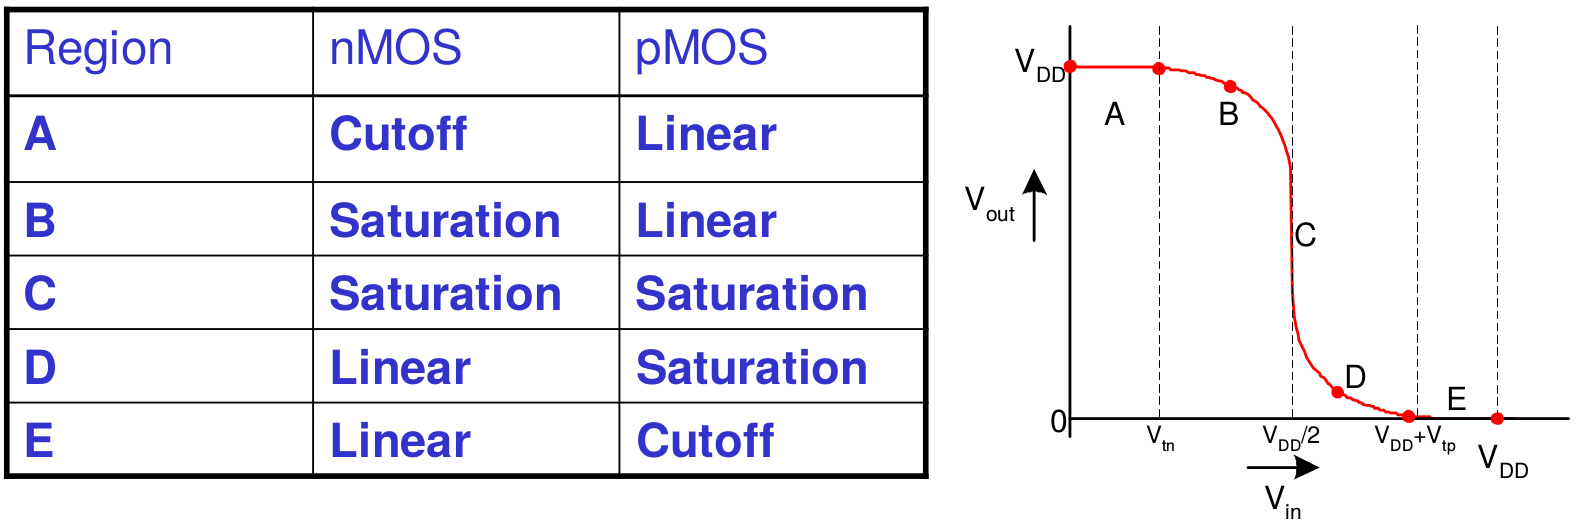
\includegraphics[width=\columnwidth]{../ecen454/DC__response_Vo_Vi_nMOS_pMOS.png}
    \2 don't want to switch nMOS and pMOS because then nMOS would saturate at far end of graph (and vice versa for pMOS)
    \2 horizontal position of graph can be varied by tuning $\beta_p / \beta_n$
      \3 called beta ratio, or skewed gate
      \3 $\beta_p / \beta_n>1 \rightarrow$ right, $\beta_p / \beta_n\rightarrow$ left
    \2 unity gain slope: part of response graph where the slope is $-1$
      \3 want to tune $\beta_p / \beta_n$ to put logic levels at these regions to maximize noise margins
    \2 Noise Margins:
      \3 $NM_H=|V_{OH}-V_{IH}|, NM_L=|V_{OL}-V_{IL}|$
      \3 that's just the higher/lower of the two axes

\zzz{Transient Analysis}
  \1 for instance, find step response of gate to determine rise time.
  \1 rise/fall delay: time from when $V_{in}$ crosses $\frac{V_{DD}}{2}$ to when $V_{out}$ crosses it
  \1 rise/fall time: (of $V_{in}$ or $V_{out}$): time for that signal to go from $0.1V_{DD}$ to $0.9V_{DD}$ (or reverse)
  \1 TODO many equations and such for inverter step response (from slides)
  \1 TODO pass transistors (form slides)

\zzz{Pass Transistors}
  \1 for nMOS trying to pass $\VDD$ or pMOS trying to pass 0
  \1 nMOS can pull no higher than $\VDD-\Vtn$ if $\Vg=\VDD$
    \2 more generally, $\Vg-\Vtn$
    \2 called degraded 1
  \1 pMOS can pull no lower than $|\Vtp|$
% end lecture 5

% lecture 6
\zzz{Delay}
  \1 generally estimated with RC models
    \2 for nMOS with width $k$:
    \2 resistance of $R/k$
    \2 caps of $kC$ on all terminals
    \2 pMOS same except resistance is $2R/k$
  \1 depends on effective $R$ and $C$ of transistors 
    \2 exactly what parasitic caps depends on exact layout (which stuff is shared between transistors)
  \1 width:
    \2 C proportional to width
     (approx 2 fF/$\mu$m)
    \2 R inversely proportional to width
      (approx 6k$\Omega$*$\mu$m)
    \2 TODO unity transistors
  \1 find widths necessary for rise and fall resistance to be same as standard inverter
    \2 pMOS is about half as conductive as nMOS, so the inverter has nMOS=1, pMOS=2
    \2 larger width $\rightarrow$ smaller $R$
    \2 transistors in series: delay adds, so double the width
    \2 transistors in parallel: same as a single transistor (because we assume worst case of only one being active)
  \1 use effective resistance in RC model: $I_{ds}=V_{ds}/R$
    (just good enough for a RC model, not for current at arbitrary time)
  \1 find delay of circuit
    \2 decompose to RC model (take into account widths of each transistor)
      \3 replace transistors with resistors
      \3 add parasitic caps on either side of every transistor (cap value = width of transistor)
        \4 caps with both pins short to ground don't count, are never charged
        \4 caps from $\VDD$ to ground don't count, always charged
    \2 add together all R and C's to get delay
      \3 don't count $R$ of nMOS and pMOS at the same time, because they're never on at the same time
  \1 \textbf{Delay} $d=f+p$
  \1 \textbf{Effort Delay} $f = gh$
    \2 $g$: logical effort: relative ability of gate to deliver current
      \3 $g=1$ for standard inverter
    \2 $h$: electrical effort: ratio of input to output capacitance
      \3 also called fanout
  \1 \textbf{Parasitic Delay} $p$
    \2 independent of load (represents delay of gate driving no load)
    \2 set by internal parasitic capacitance
  \1 Elmore Delay:
    \2 ON transistors look like resistors, so pullup/pulldown network is modeled as RC ladder
    \2 $t = \sum_{i\in nodes} R_{i-to-source}C_i$
    $= R_1C_1 + (R_1+R_2)C_2+\ldots+(R_1+\ldots+R_n)C_n$
  \1 Ideal number of stages for inverter driving large load
    \2 delay $ = \left( \frac{C_{load}}{C_{inv}} \right) ^\frac{1}{k} k R_{inv} C_{inv}$
    \2 $k$: number of stages
    \2 stage size ratio: $\left( \frac{C_{load}}{C_{inv}} \right) ^\frac{1}{k}$

\zzz{Static Timing Analysis}
  \1 worst case at each step
  \1 in form arrival time / required arrival time / slack
  \1 arrival time: input to output, take max
  \1 required arrival time: output to input, take min
    \2 work backward
    \2 if a gate drives only one gate on it's output, this is trivial
  \1 slack: required arrival time $-$ arrival time
  \1 Contamination delay: just best case delay (smallest delay)
    \2 in this case, you'll count parallel transistors as parallel resistors
  \1 not sure about this stuff, Peter just said to not worry about this question on the homework

\zzz{Power Estimation}
  \1 Dynamic Power
    \2 power required to charge the load capacitor
    \2 only counted when transistor switches
      \3 therefore this power usage is data dependent
      \3 therefore, you have to count the falling transitions in the output per time period
    \2 $P_{dynamic} = \frac{1}{T}\int_0^T i_{DD}(t) \VDD dt$
    \2 for any gate: $P_{dynamic} = C \VDD^2 f_{sw}$
  \1 Activity Factor $\alpha$
    \2 $\alpha$: how often this gate switches in terms of the base clock frequency
    \2 $\alpha=1$: clock; $\alpha=0.5$: every other cycle, etc...
    \2 for system clock at frequency $f$, $P_{dynamic} = \alpha C \VDD^2 f$
  \1 Short Circuit Current
    \2 nMOS and pMOS may both be on for a short instant during switching, leading to a short instant of short circuit current (from $\VDD$ to ground)
    \2 $P_s \propto (\VDD -2V_t)^3 t_r f_p$
      \\ assume $t_r=t_f$ for input
      \\ $f_p$: frequency of input
    \2 this is less than $10\%$ of dynamic power if the rise/fall times are comparable
  \1 Static Power
    \2 leakage when gate is off
    \2 
    $$ I_{ds} = I_{ds0} e^{\frac{\Vgs-\Vt}{nv_T}} \left( 1 - e^{\frac{-\Vds}{v_T}} \right) $$
    $$ V_t = V_{t0} - \eta\Vds + \gamma \left( \sqrt{\phi_s + V_{sb}} - \sqrt{\phi_s} \right) $$


    







\zzz{After exam 1}
  \1 exam 1 was on March 8 (2017.03.08)
  \1 nothing specifically from previous exam

\zzz{Propagation vs Contamination delay}
  \1 contamination delay ($t_{cd}$): time from input change to \textbf{any} output changing value
    \2 kind of a best-case delay or smallest possible delay
    \2 time counted when input crosses 50\% of logical high voltage level
  \1 propagation delay: time from when all inputs are stable to when all outputs are stable
    \2 kind of like a worst-case delay

\zzz{Latch vs Flip Flop}
  \1 Latch is level-sensitive, flip-flop is edge-sensitive
  \1 register is flip-flop
\zzz{Latch/flip flop designs}
  \1 pass transistor latch
    \2 pros: tiny, low clock load
    \2 con: voltage drop across is $V_t$, it's non-restoring
    \2 con: not really a latch because doesn't hold signal
  \1 transmission gate
    \2 pro: no $V_t$ drop
    \2 con: requires inverted clock
  \1 inverting buffer
    \2 TODO
  \1 tristate feedback
    \2 first complete latch here
    \2 risk of backdriving: downstream could change state if it is very strong
  \1 buffered output
    \2 no backdrifing problem
    \2 widely used
    \2 rather large and slow though, and large load on clock
  \1 a flip-flop is just two latches back-to-back

\zzz{Metastability}
  \1 stable works if it's not at a strong high or low but will settle somewhere
  \1 metastable is where it might sit there, but if it must settle, you don't know which one it will settle to when perturbed

% 2017.03.27
\zzz{Sequential Circuits}
  \1 sequential means that the circuit holds state: the output depends on both current and past input
  \1 to model a state machine, you can unroll it to [regieter] $\rightarrow$ [combinational] $\rightarrow$ ...
    \2 this way you can use regular timing stuff for it: arrival time, slack, etc...
  \1 Mealy FSM: output of circuit is from combinational logic
  \1 Moore FSM: output is from registers
  \1 pipelined circuit: uses registers to hold state between clock cycles, because not all of the combinational logic can happen fast enough to work in a single clock cycle
    \2 pipelined circuits can use flip-flops or latches?
  \1 the clock consumes 20-30\% of the power on a chip
  \1 the whole reason that registers are needed is because data (signals) moves through components at non-constant speed
  \1 reset
    \2 can be sync or async
    \2 force low output when reset is high
  \1 sequencing: it is (generally) equivalent to split the sequential logic in two, and then use two latches (one halfway through) instead of one large section of sequential logic with flip-flops at either end
    \2 this is called two phase clocking
    \2 you have to make sure the middle latch operates on clock-bar instead of clock
  \1 timing: \\
  \begin{tabular}{l l}
    $t_{pd}$ & logic propagation delay \\
    $t_{cd}$ & logic contamination delay \\
    $t_{pcq}$ & Clk$\rightarrow$Q propagation delay \\
    $t_{ccq}$ & Clk$\rightarrow$Q contamination delay \\
    $t_{pdq}$ & D$\rightarrow$Q propagation delay \\
    $t_{setup}$ & setup time \\
    $t_{hold}$ & hold time \\
  \end{tabular}
    \2 D$\rightarrow$Q delay only makes sense for latches, since for flip-flops it is simply one clock cycle
  \1 sequencing overhead: TODO
  \1 time borrowing: TODO









% lecture 8? (HW7)

\zzz{Wire Delay}
  \1 $n$-segment $\pi$ model:
  \\ to model, find total R and C of wire; then split up according to $n$ segment model, then combine adjacent caps

\zzz{Miller Effect}
  \1 AKA crosstalk; it's when one wire affects another
  \1 it's dynamic; depends on what signal the wires are carrying
  \1 MCF: Miller factor (or something)
  \1 for two wires A and B, model as $C_{eff} = C_{gnd} + MCF \cdot C_{adj}$
  \1 MCF: \begin{tabular}{l|l}
  behavior of B & MCF \\ \hline
  constant   & 1 \\
  with A     & 0 \\
  opposite A & 2 \\
  \end{tabular}

\zzz{Timing}
  \1 setup time: minimum time that signal must remain stead \textbf{before} clock edge
  \1 hold time:  minimum time that signal must remain stead \textbf{after}  clock edge
  \1 propagation delay: when driving another gate? largest (worst case) delay?
  \1 contamination delay: best case delay (smallest delay)?
  \1 parasitic delay: independent of load
  \1 effort delay: proportional to load capacitance (nothing to do with the thing that is doing the driving of the load capacitance)
  \1 maximum possible logic propagation delay for combinational circuit buffered on either side by flip-flops:
    clockCycle - Clk$\rightarrow$Q - FlipFlopSetup - WorstSkew
    \2 minimum circuit delay: HoldTime - Clk$\rightarrow$Q

\zzz{Memory}
  \1 serial access memory (SAM): accessed in a sequence, not randomly
    \2 ex. shift register, queue, stack, etc...
    \2 often implemented using random access memory
  \1 Shift Register
    \2 serial in, parallel out
    \2 large number of transistors per cell when implemented using flip flop
    \2 tapped delay line: shift register with variable number of stages
      \3 useful for allowing chips at different clock frequencies to communicate (apparently)
  \1 queue or stack can be built using SRAM block with pointers to first/last and stuff
  \1 SRAM
    \2 static ram
    \2 can be dual ported: means you can write to a cell while reading the old value from it
    \2 designed in a cell grid, MUXes for input and then decoders for output connected to bit lines that run across the cells
    \2 TODO note about pre charging bit line
  \1 DRAM
    \2 stores bits using capacitors
  \1 decoders
    \2 needed to switch to the right bit-line
    \2 need to be pitch-matched to RAM cell width for efficiency
    \2 TODO note about twisted bit lines
  \1 ROM: read only memory
    \2 used to be custom masked chips for data
    \2 
  \1 PROM


\zzz{Packaging}
  \1 flip chip: put connection pads on the surface of the die instead of the edges
    \2 then flip the chip over and affix it directly to the package
    \2 means the die must be positioned in the package more precisely
  \1 Heat
    \2 Thermal Resistance: $\Delta T = \theta_{jaa} P$
      \3 $\Delta T$: temperature rise in chip
      \3 $\theta_{ja}$: thermal resistance of chip junction to ambient; units: $C/W$
      \3 $P$: power dissipation on chip
  \1 IO
    \2 ESD Protection: TODO
    \2 output pads:
      \3 must drive large off-chip loads (2-50pF)
      \\ do that using successively larger buffers
      \3 surround with guard ring to protect against lockup
    \2 input pads:
      \3 may need level converters
      \3 Schmitt trigger: allow signal to cross high/low edge only after it goes a little over the tipping point
    \2 bidirectional pads:
      \3 combine input and output
      \3 use tristate driver to set pin direction
    \2 analog:
      \3 no buffering
      \3 any protection circuitry must be careful to not distort the signal at all
      \3 RF pads?


\end{outline}
\end{flushleft}
\end{multicols*}
\end{spacing}
\end{document}

